%%%%%%%%%%%%%%%%
% Set options

\newcommand{\mpnumber}{mp5}
\newcommand{\settitle}{Project 5: Forensics}
\newcommand{\course}{CS461/ECE422}
\newcommand{\coursename}{Computer Security I}
\newcommand{\duedate}{Wednesday, May 4}
\newcommand{\checkpointduedate}{Monday, April 25}
\newcommand{\duetime}{6:00pm}
\newcommand{\distdate}{April 18, 2015}
\newcommand{\semester}{Spring 16}
\newcommand{\firstcheckpointpercent}{2\%}
\newcommand{\secondcheckpointpercent}{10\%}
\newcommand{\staffemail}{\textbf{ece422-staff@illinois.edu}}
\newcommand{\svnrepo}{https://subversion.ews.illinois.edu/svn/sp16-ece422}
\newcommand{\forensicsfile}{forensics\_sp16\_victim}

%%%%%%%%%%%%%%%%

\documentclass[letterpaper,12pt]{report}
\usepackage{fullpage}
\usepackage[protrusion=true,expansion=auto]{microtype}
\usepackage{color}
\usepackage[T1]{fontenc}
\usepackage{lmodern}
\usepackage{mathptmx}
\usepackage{textcomp}
\usepackage{fancyvrb}
\usepackage{listings}
\usepackage{paralist}
\usepackage{url}
\usepackage[
  breaklinks=true,colorlinks=true,linkcolor=black,%
  citecolor=black,urlcolor=black,bookmarks=false,bookmarksopen=false,%
  pdfauthor={\course},%
  pdftitle={\settitle},%
  pdftex]{hyperref}
\usepackage{amsmath}
\usepackage{amsfonts}
\usepackage{multicol}
\def\textsb#1{{\fontseries{sb}\selectfont #1}}
\usepackage{mdframed}
\usepackage{graphicx}
\usepackage{float}
\graphicspath{{./figures/}}
\setcounter{secnumdepth}{3}

\newcommand{\problemsetdone}{\bigskip\hfill$\Box{}$}

\newcommand{\htitle}
{
     \noindent\parbox{\textwidth}
    {
        \course\hfill \distdate\newline
        \coursename\hfill 
        \settitle \vspace*{-.5ex}\newline
        \mbox{}\hrulefill\mbox{}
    }
    \vspace{8pt}
    \begin{center}{\Large\bf{\settitle}}\end{center}
}
\newcommand{\handout}
{
    \thispagestyle{empty}
    \markboth{}{}
    \pagestyle{plain}
    \htitle
}

\newcommand{\problemsetheader}
{
\setlength{\parindent}{0pt}

\medskip

This project is split into two parts, with the first checkpoint due on {\bf \checkpointduedate} at {\bf \duetime} and the second checkpoint due on {\bf \duedate} at {\bf \duetime}. The first checkpoint is worth {\firstcheckpointpercent} of your total grade, and the second checkpoint is worth \secondcheckpointpercent.  We strongly recommend that you get started early. Each semester everyone will be given ONE late extension that allows you to turn in up to one assignment(checkpoint) up to 24 hours after the due date. Extensions are not automatic. So, if you want to use your late extension, you MUST send an e-mail to {\staffemail}. Late work will not be accepted after 24 hours past the due date. 

\medskip

\textbf{Start early}. It may be impossible to complete this project before the deadline unless you begin several days beforehand. Please plan accordingly.

\medskip

This is a group project; you SHOULD work in \textbf{teams of two} and if you are in teams of two, you MUST submit one project per team.  Please find a partner as soon as possible.  If have trouble forming a team, post to Piazza's partner search forum.

\medskip

Not all groups will finish all the tasks in all the MPs. The tasks in each MP are designed to be progressively harder with the final tasks in each MP having been designed as *significant* challenges. Some difficult tasks are placed earlier for better understanding of the scenario flow.

\medskip

\textbf{Strict \underline{NO-leaks} policy.}  In this project you play the role of a computer forensic analyst working to solve a murder case.  Since you don't want to be fired for jeopardizing an ongoing criminal investigation, you need to follow a strict policy on collaboration.  \emph{You are bound by the Student Code not to communicate with anyone regarding any aspect of the case or your investigation (other than within your group or with course staff)}.  The number of pieces of evidence you find, the techniques you try, how successful said techniques are, the general process you follow, etc.\ are all considered part of your solution and must not be discussed with members of other groups.

\medskip

Solutions MUST be submitted electronically in any one of the group member's svn directory, following the submission checklist given at the end of each checkpoint. Details on the filename and submission guideline is listed at the end of the document.

\medskip

\hrulefill

\medskip
}

%%%%%%%%%%%%%%%%%%%%%%%%%%%%%%%%%%%%%%%%%

\begin{document}
\handout
%\setlength{\parindent}{0pt}
\problemsetheader
\medskip
\noindent
\emph{``In general, computer forensics is rather ad hoc. Traditional rules of evidence are broken all the time. But this seems like a pretty egregious example."}

~~~~~~~~~~~~~~~~~~~~~~~~~~~~~~~~~~~~~~~~~~~~~~~~~~~~~~~~~~~~~~~~~~~~~~~-- Bruce Schneier 

\newpage

\section*{Introduction}

In this project, you will play the role of a digital forensic analyst and investigate a murder mystery. 

\medskip

A few days after Halloween 2015, a terrible crime occurred on University of Illinois at Urbana Champaign campus.
Hapless Victim was murdered in the dorm. Victim was last seen alive on November 4, 2015 early afternoon in class,
and was discovered dead at approximately 11pm the same day. 

\medskip

Officers were not able to immediately detect the actual sign of the death and asked forensics team to investigate.
While waiting for forensics team to share the result, they have performed digital forensics analysis on victim's hard disk.
A suicidal note was left on the hard disk. Forensics team confirmed that the victim was dead as how the suicidal note mentioned.
Hence, investigation department's initial conclusion to the case was suicidal.

\medskip

However, with further investigation, they opened the possibility of murder and filtered out few suspects.
They could not find all suspects, but instead, were able to obtain the hard disk of all suspects.
Investigators successfully decrypted the hard disks and created image for further investigation.

\medskip

Your job is to conduct a forensic examination of the disk image and document any evidence related to the murder. 
If you find sufficient evidence, the suspect will be extradited and face trial.

\section*{Objectives}
\begin{itemize}
\item Understand how computer use can leave persistent traces and why such evidence is often difficult to remove or conceal.
\item Gain experience applying the security mindset to investigate computer misuse and intrusion.
\item Learn how to retrieve information from a disk image without booting the operating system, and understand why this is necessary to preserve forensic integrity.
\end{itemize}

\section*{Guidelines}
\begin{itemize}
\item You SHOULD work in a group of 2.
\item Your answers may or may not be the same as your classmates'.
\item All the necessary files to start the project will be given under the folder called ``\mpnumber'' in your SVN repository: \url{\svnrepo/NETID/\mpnumber}.
\item We generated files for you to submit your answers in.  You MUST submit your answers in the provided files; we will only grade what's there!
\item Each submission file contains an example of expected format. Failure to follow this format may result in autograder failure. You MAY delete the examples; they will be ignored (along with any other line starting with \#) when grading.
\item Solution format is case-insensitive.
\end{itemize}

\section*{Read this First}
\paragraph{Collaboration: Strictly prohibited outside your group.}
As stated above, you are bound by the Student Code not to communicate with anyone regarding any aspect of the case or your investigation (other than within your group or with course staff).  The number of pieces of evidence you find, the techniques you try, how successful said techniques are, the general process you follow, etc.\ are all considered part of your solution and must not be discussed with members of other groups.  If anyone brings up the project, put your fingers in your ear, start yelling ``LALALALA'', run around and refer them to your supervisor for an official spokesperson.

\newpage

\section*{Getting Started}

Tools and techniques you use for your investigation are up to you, but here are some suggestions to help you get started. This MP requires multiple tools to be downloaded and installed and you MUST use your own system. EWS is not supported for this MP: 1) Virtual Machine is not allowed, 2) generating files: decompressed disk image and virtual hard disk image, sums up to >10GB which exceeds allocated quota, 3) Autopsy version installed doesn't support our VM file system, 4) password-cracking software should be run on private computer. Finally, we \textbf{strongly recommend to use Autopsy on Windows OS} as it provides extra functions which pre-filters interesting evidence and will tremendously save your investigation time.

\paragraph{General Knowledge}
 A general working knowledge of Linux is undoubtedly helpful for this project. If you don't have this yet, you may need to spend time Googling and/or experimenting to get up to speed. The TA will also answer general Linux questions as a last resort.  For an excellent reference book, try \emph{UNIX and Linux System Administration Handbook} by Nemeth, Snyder, Hein, and Whaley.  Ebook can be found at \url{\svnrepo/\_shared/\mpnumber/unix\_system\_handbook.pdf}.  Also, see \url{http://en.wikipedia.org/wiki/Disk\_partitioning}\ for some additional background.

\paragraph{Live Analysis}
Live analysis is a forensic technique in which the investigator examines a running copy of the target system.  We suggest using VirtualBox for this purpose.

\begin{enumerate}
\item Download the compressed raw disk image (1.5~GB):
    \begin{sloppypar}
    \texttt{\$ wget \url{\svnrepo/\_shared/\mpnumber/\forensicsfile.raw.gz}}
    \end{sloppypar}
\item Decompress the disk image.\\
    \texttt{\$ gunzip \forensicsfile.raw.gz}
\item Download the checksum file. This contains two different checksums: compressed (raw.gz) and decompressed (raw) files. If either of the checksums matches, you are good to proceed.
    \begin{sloppypar}
    \texttt{\$ wget \url{\svnrepo/\_shared/\mpnumber/SHA256SUMS.txt}}
    \end{sloppypar}
\item Verify the checksum. You can repeat this process for checkpoint 2 VM.\\
    \texttt{On Linux: \$sha256sum -c SHA256SUMS.txt}\\
    \texttt{On OS X:  \$shasum -a 256 -c SHA256SUMS.txt}
\item Convert the raw disk image to a VirtualBox disk image:\\
    \texttt{\$ VBoxManage convertdd \forensicsfile.raw forensics.vdi --format VDI}
\item Use the VirtualBox GUI to create a new VM.  Select Linux / Ubuntu (32-bit) as the machine type.  Select ``Use an existing virtual hard disk file'' and select the VDI you just created.
\item Start the VM and explore the system.
\end{enumerate}

\paragraph{Dead Analysis}
In dead analysis, forensic investigator examines data artifacts from a target system without running the system. We suggest trying dead analysis with the Autopsy open-source forensics tool. The procedure below assumes you are working on Ubuntu Linux. Autopsy will also run on Windows and OS~X. For OS~X, Sleuth Kit should be installed prior to Autopsy installation.  Sleuth Kit can be downloaded from \url{http://www.sleuthkit.org/sleuthkit/download.php}.

\begin{enumerate}
\item Compile and install the Autopsy digital forensics suite: visit below link and follow the instruction.\\
    \url{http://www.sleuthkit.org/autopsy/download.php}\\ \\
    \textit{Note:} Do not install using ``apt-get'' command. The version available from apt-get is Autopsy 2.24, which doesn't support ext4. Our VM is based on ext4 which is unable to show all file system on version under 3.0.6. Make sure to download version 4.0.0 and compile.
% \item If you are using EWS Linux machine, load sleuth kit:\\
% 	\texttt{\$ module load sleuthkit}
\item Launch Autopsy in the background and open the browser-based GUI:\\
    \texttt{\$ sudo autopsy \&}\\
    In a browser on the local machine, go to the URL \url{http://localhost:9999/autopsy}.
\item Create a new case and add the disk image:
    \begin{enumerate}
        \item Click New Case.  Enter a case name and click New Case.
        \item Go back to \url{http://localhost:9999/autopsy} and open the case you created.
        \item Click Add Host.  Enter a host name and input the time zone of the system to analyze. If time zone is not specified, it will use your computer system time zone by default. Click Add Host.
        \item Click Add Image.  Click Add Image File.  Enter the path to the decompressed raw disk image.  Make sure you select  Type=Disk and Import Method=Symlink.  Click Next.
        \item Leave the Image File Details and File System Details as the defaults.  (Note that the disk image contains 3 partitions, which Autopsy will allow you to examine separately.)  Click Add.  Click OK.
        \item Select a partition to examine and click Analyze.  The buttons at the top give you several analysis tools.  Try File Analysis and Keyword Search to get started.
    \end{enumerate}
\item In addition to hints dropped elsewhere, here is an incomplete list of things to try: 
    \begin{itemize}
        \item Examine the system logs.
        \item Check for deleted or encrypted files.
        \item Search the drive image for strings that may indicate relevance to your investigation.
    \end{itemize}

\end{enumerate}

\textbf{Note:} If you are having issues with image mounting procedure (or mounts successfully but fails to provide the correcting mounting point), you may not see all file systems and directories with above instructions, so try below alternative. 

\medskip
This procedure will not completely replace Autopsy as you will need to do all the analysis/searches manually. You should find another operating system to run Autopsy properly.

\begin{enumerate}
    \item Create a directory where you will mount the image.\\
        \texttt{\$ sudo mkdir /mnt/victim}
    \item Mount the image to the mount directory you created.
        \begin{sloppypar}
        \texttt{\$ sudo mount -t ext4 -o loop,ro,noexec,offset=1048576 [raw\_image\_file\_path] /mnt/victim}
        \end{sloppypar}
        This command mounts the specified image to the specified location as a loop, read-only, no-execute ext4 (the filesystem that linux commonly uses) partition. 
        The offset needs to be specified because your host system will not know exactly at where the linux partition resides within that disk image. 
        The offset is 1048576 because the partition starts at sector 2048, and each sector is 512 bytes. 2048 * 512 = 1048576.
    \item Once the image is mounted, you can pretty much browse that partition as if it's part of your own filesystem.
    \item Change directory to the mount directory.\\
        \texttt{\$ cd /mnt/victim[or full\_path\_to\_the\_directory\_you\_created]}
    \item List the files in the directory. You will see files and folders that are similar to your root directory.\\
        \texttt{\$ ls}
\end{enumerate}

\paragraph{Password Cracking}
Password crackers may be helpful in trying to brute-force decrypt password-protected files.  Not all the tools will be used for this MP exploration, but here are some useful tools list.  John the Ripper (\url{http://www.openwall.com/john/}) is the canonical Unix password cracker.  Hydra  (\url{http://www.thc.org/thc-hydra/}) is a tool used to brute force remote login passwords, fcrackzip (\url{http://home.schmorp.de/marc/fcrackzip.html}) is a ZIP password cracker, and pdfcrack (\url{http://sourceforge.net/projects/pdfcrack/}) is a PDF password cracker. John, fcrackzip, and pdfcrack are conveniently available in the Debian package repositories and can be installed with \texttt{apt-get}.

\medskip

When using a password cracker, it is wise to make sure that the password is not susceptible to a dictionary attack and does not use a restricted character set (e.g., lowercase letters, letters only, letters and numbers only) before spending time on a full brute-force crack. It is also a good idea to crack a very vulnerable password first to make sure you are using the tool correctly.

\paragraph{Metadata Viewer}
There exists multiple metadata viewer, but for our MP, we will be using ExifTool by Phil Harvey. It can be downloaded at (\url{http://owl.phy.queensu.ca/~phil/exiftool/}). Follow the instructions on the website to view the metadata of the evidence. 

\newpage

%Set counter for MP number
\setcounter{chapter}{5}

\section{Checkpoint 1 (20 points)}
\label{sec:checkpoint_1}

The deliverables for this project are your answers to the questions below. Your answers should be \emph{complete} but \emph{concise}.

\medskip 

For each prompt, you may optionally explain the investigatory methods you used and the evidence that supports your conclusion.  The files can be included in a separate directory named \texttt{explanation/}.  These explanations will not be graded but can be considered during manual regrading.

\section*{Exploring Victim's Traces}
\label{sec:victim_traces}
In this part of the project, you will be exploring the traces left on victim's hard disk.

\subsection{Username (2 points)    \hfill\rm\normalsize (\emph{Difficulty: Easy})}
\label{sec:username}
What is the username of the victim used on OS?

\medskip 
\textbf{What to submit:} Submit a text file named \texttt{\ref{sec:username}.txt} that contains the username of the victim.

\medskip
\textit{Note:} Username is the id used to log on to the system. For example, there is a student, \texttt{Yann Simpson}, whose netid is \texttt{yann}. To access the University system, the netid, \texttt{yann} is used as username to log on. If logged on, they will display either the netid or the full name to indicate the user of the account. Illustrative example is shown below.

\begin{figure}[H]
  \centering
  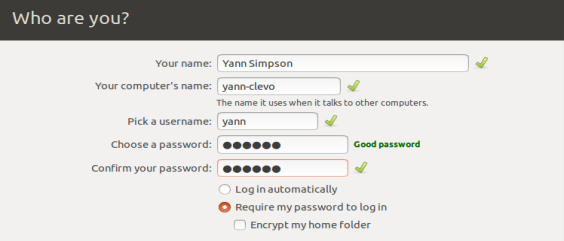
\includegraphics[width=0.6\textwidth]{unix_username.png}
\end{figure}

\subsubsection*{example content of {\ref{sec:username}.txt}}
\begin{mdframed}
\begin{Verbatim}
# this line is ignored
yann
\end{Verbatim}
\end{mdframed}

\subsection{Timezone (2 points)    \hfill\rm\normalsize (\emph{Difficulty: Easy})}
\label{sec:timezone}
What is the timezone setting of the victim's system? 

\medskip 
\textbf{What to submit:} Submit a text file named \texttt{\ref{sec:timezone}.txt} that contains the timezone of the victim's system.

\medskip
\textit{Hint:} The system is based on one of US time zones. Four time zones in US are EST, CST, MST, and PST. Do NOT submit in any other format, e.g. UTC, America/New York, Eastern Time Zone etc.

\subsubsection*{example content of {\ref{sec:timezone}.txt}}
\begin{mdframed}
\begin{Verbatim}
EST
\end{Verbatim}
\end{mdframed}

\subsection{Conversation (4 points)    \hfill\rm\normalsize (\emph{Difficulty: Easy})}
\label{sec:conversation}
Whom did the victim have conversation(s) with? List each username in separate line, in the order of occurrences. 

If the victim had multiple conversations with the same person in different times, list the username as many as the conversation history. Note that this does not equal to the message count transferred back and forth for single conversation.

\medskip 
\textbf{What to submit:} Submit a text file named \texttt{\ref{sec:conversation}.txt} that contains the list of usernames the victim have conversation with in chronological order.

\medskip
\textit{Note:} For example, let's assume that Alice is a victim and you are exploring the chat history. The list below is the summary of the chat histories you have explored. Then, the solution to this example will be the following.
 
\medskip
\texttt{<Alice's chat history>\\
        (with bob@chat.org) @ Apr 2 7:00pm\\
        (with eve@chat.org) @ Apr 3 10:00am\\
        (with eve@chat.org) @ Apr 3 2:00pm}

\subsubsection*{example content of {\ref{sec:conversation}.txt}}
\begin{mdframed}
\begin{Verbatim}
bob
eve
eve
\end{Verbatim}
\end{mdframed}

\subsection{Evidence file (4 points)    \hfill\rm\normalsize (\emph{Difficulty: Easy})}
\label{sec:evidence_file}
The police initially thought that the victim committed suicide after finding a certain file on the victim's computer.

\begin{enumerate}
\item What is the name of the file? Include the file extension.
\item When was this file last modified? Submit the time in MMddhhmm 24-hr format. (MM=Month, dd=day, hh=hour, mm=minute). For example, 11:30pm on April 3rd is 04032330.
\end{enumerate}

\paragraph{What to submit}
\begin{enumerate}
\item Submit a text file named \texttt{\ref{sec:evidence_file}\_name.txt} that contains the full name of the file.
\item Submit a text file named \texttt{\ref{sec:evidence_file}\_time.txt} that contains the last modified time of the file.
\end{enumerate}

\subsubsection*{example content of {\ref{sec:evidence_file}\_name.txt}}
\begin{mdframed}
\begin{Verbatim}
evidencefile.txt
\end{Verbatim}
\end{mdframed}

\subsubsection*{example content of {\ref{sec:evidence_file}\_time.txt}}
\begin{mdframed}
\begin{Verbatim}
04032330
\end{Verbatim}
\end{mdframed}

\subsection{Attack (8 points)    \hfill\rm\normalsize (\emph{Difficulty: Medium})}
\label{sec:attack}
After initial conclusion, the police started to be suspicious about possibility of the murder. Do you find any trace of the attack on victim's machine? 

\begin{enumerate}
\item If so, when did the attacker make the first contact to the victim's computer? Any contact can either be successful login or failed attempt. Submit the time in MMddhhmm 24-hr format. (MM=Month, dd=day, hh=hour, mm=minute).
\item List all the IP addresses the attack originated from. Submit IPv4 addresses. If there are multiple attacker IP addresses, include one IP address per each line.
\item What was the victim's IP address during the attack? Submit IPv4 address.
\end{enumerate}

\paragraph{What to submit}
\begin{enumerate}
\item Submit a text file named \texttt{\ref{sec:attack}\_time.txt} that contains the first attack time.
\item Submit a text file named \texttt{\ref{sec:attack}\_attackerip.txt} that contains the list of IP addresses the attack came from.
\item Submit a text file named \texttt{\ref{sec:attack}\_victimip.txt} that contains the victim's IP address.
\end{enumerate}

\subsubsection*{example content of {\ref{sec:attack}\_attackerip.txt}}
\begin{mdframed}
\begin{Verbatim}
1.2.3.4
5.6.7.8
\end{Verbatim}
\end{mdframed}

\newpage

\section*{Checkpoint 1: Submission Checklist}

Inside your \texttt{\mpnumber} directory svn, you will have the auto-generated files named as below.  Make sure that your answers for all tasks up to this point are submitted in the following files before \textbf{\checkpointduedate} at \textbf{\duetime}:

\subsection*{SVN Directory}
\url{\svnrepo/NETID/\mpnumber}

\begin{itemize}
\item {\tt partners.txt} [One netid on each line]
\item \texttt{\ref{sec:username}.txt}
\item \texttt{\ref{sec:timezone}.txt}
\item \texttt{\ref{sec:conversation}.txt}
\item \texttt{\ref{sec:evidence_file}\_name.txt}
\item \texttt{\ref{sec:evidence_file}\_time.txt}
\item \texttt{\ref{sec:attack}\_time.txt}
\item \texttt{\ref{sec:attack}\_attackerip.txt}
\item \texttt{\ref{sec:attack}\_victimip.txt}
\end{itemize}


\newpage

\section{Checkpoint 2 (100 points)}
\label{sec:checkpoint_2}
The deliverables for this project are your answers to the questions below. Your answers should be \emph{complete} but \emph{concise} following the submission template.

\medskip
Suspect VM that you will explore is given individually in your SVN directory. Follow and download the disk image provided in \texttt{suspect\_vm.txt}. We have also created \texttt{code.txt} in your SVN directory. The instruction for this file will be given at some point in the project, so be patient.

\medskip
If you recover files that are relevant to your responses, include them with your submission in a directory named \texttt{evidence/}. Do not change the original file name on your submission.
For each prompt, you may optionally explain the investigatory methods you used and the evidence that supports your conclusion.  The files can be included in a separate directory named \texttt{explanation}.

\section*{Investigating Suspect Traces}
In this part of the project, you will be exploring the traces left on suspect's hard disk.

\subsection{Live Analysis (10 points)    \hfill\rm\normalsize (\emph{Difficulty: Hard})}
\label{sec:live_analysis}
Now, the police department has obtained multiple suspects' hard disk, distributed them across teams to be investigated in parallel. You are given with one disk image to analyze. Answer the following set of questions to fill out the report.

\medskip
You were given with one disk image to analyze. Now, you want to try the live analysis of the evidence. You must perform live analysis to answer subset of questions, but you can also perform dead analysis to obtain the evidence.

\medskip
Let's first take a look at the machine environment. Be careful and specific; e.g., say ``Windows 2000'' instead of just ``Windows.''

\begin{enumerate}
\item Try booting the suspect's machine and using it normally. What operating system does it boot by default? Include OS name and the distribution release number in separate lines. 
\item What specific or potentially dangerous behavior(s) of the default boot OS have on the machine? Find a script that executes the specific behavior. Submit the name of the script file.
\item What operating system did the suspect primarily use? Submit the OS's name and distribution release number in separate lines.
\end{enumerate}

\paragraph{What to submit}
\begin{enumerate}
\item Submit a text file named \texttt{\ref{sec:live_analysis}\_default.txt} that contains the default booting OS.
\item Submit a text file named \texttt{\ref{sec:live_analysis}\_behavior.txt} that contains the script file name that executes the specific behavior of the default booting OS.
\item Submit a text file named \texttt{\ref{sec:live_analysis}\_primary.txt} that contains the primary OS the suspect used.
\end{enumerate}

\medskip
\begin{sloppypar}
\textit{Note:} Note that OS distribution number is not equivalent to the kernel number. Refer the details at \url{http://whatsmyos.com/} or \url{https://www.linux.com/learn/tutorials/824791-how-to-find-your-linux-version-or-distro-release-and-why-it-matters}.
\end{sloppypar}

\subsubsection*{example content of {\ref{sec:live_analysis}\_\{default,primary\}.txt}}
\begin{mdframed}
\begin{Verbatim}
OS X
10.10.4
\end{Verbatim}
\end{mdframed}

\subsubsection*{example content of {\ref{sec:live_analysis}\_behavior.txt}}
\begin{mdframed}
\begin{Verbatim}
scriptfile.ext
\end{Verbatim}
\end{mdframed}


\subsection{Dead Analysis (90 points)}
\label{sec:suspect_traces}
We have explored some system details through live analysis in section \ref{sec:live_analysis}. There can be potential risks during live analysis and the act may contaminate the evidence. For this section, you will be strictly performing the dead analysis to complete the investigation.

\medskip
Now, with the same disk image you have performed live analysis in the section \ref{sec:live_analysis}, you will mount on Autopsy and explore without turning on the system. Answer the following set of questions to fill out the report.

\subsubsection{Username (5 points)    \hfill\rm\normalsize (\emph{Difficulty: Easy})}
\label{sec:username_suspect}
What is the OS username of the suspect?

\medskip 
\textbf{What to submit:} Submit a text file named \texttt{\ref{sec:username_suspect}.txt} that contains the OS username of the suspect.

\subsubsection{Conversation (5 points)    \hfill\rm\normalsize (\emph{Difficulty: Easy})}
\label{sec:conversation_suspect}
You have investigated conversation history of the victim in section \ref{sec:victim_traces}. Now, you will do the same for the suspect.

\begin{enumerate}
\item Whom did the suspect have conversation(s) with? List each username in separate line, in the order of occurrences. If the suspect had multiple conversations with the same person in different times, list the username as many as the conversation history. Note that this does not equal to the message count transferred back and forth for single conversation. Note: Consider only the chat history similar to checkpoint 1.
\item What is the suspect's relationship with the victim? Choose the most appropriate one among following choices. Submit just the alphabet of the choice.
    \begin{enumerate}
        \item victim's best friend who liked victim's girlfriend
        \item victim's girlfriend
        \item victim's boyfriend
        \item course instructor who received bad feedback from victim
        \item boyfriend of the girl whom victim cheated with
        \item victim's course project partner who had to do all the work by himself/herself
        \item none of the above
    \end{enumerate}
\end{enumerate}

\paragraph{What to submit}
\begin{enumerate}
\item Submit a text file named \texttt{\ref{sec:conversation_suspect}\_usernames.txt} that contains the list of usernames the suspect have conversation with.
\item Submit a text file named \texttt{\ref{sec:conversation_suspect}\_relationship.txt} that contains the relationship of the suspect and the victim.
\end{enumerate}

\subsubsection*{example content of {\ref{sec:conversation_suspect}\_relationship.txt}}
\begin{mdframed}
\begin{Verbatim}
# alphabet of the choice
k
\end{Verbatim}
\end{mdframed}

\subsubsection{Search History (10 points)    \hfill\rm\normalsize (\emph{Difficulty: Medium})}
\label{sec:search_history}
There must be a reason that the user is considered as suspect.

\begin{enumerate}
\item Are there any indications that the suspect was trying to make an attack? How about any indication that the suspect owned or was researching weapons of the kind involved in the murder? What are the websites suspect visited potentially related with murder? List 5 website full links, one link per line in time order. They all have to come from different domains. E.g. Two different searches on Google count as 1. Don't forget to check the typos and whether all letters included.
\item What did the suspect plan to use as a weapon to murder the victim? Note that the toy evidence included in this case is considered lethal and dangerous.
\end{enumerate}

\paragraph{What to submit}
\begin{enumerate}
\item Submit a text file named \texttt{\ref{sec:search_history}\_link.txt} that contains the list of websites visited related with the murder.
\item Submit a text file named \texttt{\ref{sec:search_history}\_weapon.txt} that contains the weapon that suspect planned to use.
\end{enumerate}

\newpage

\subsubsection*{example content of {\ref{sec:search_history}\_links.txt}}
\begin{mdframed}
\begin{Verbatim}
https://www.google.com/maps
https://www.cnet.com/news/
\end{Verbatim}
\end{mdframed}

\subsubsection*{example content of {\ref{sec:search_history}\_weapon.txt}}
\begin{mdframed}
\begin{Verbatim}
lightsaber
\end{Verbatim}
\end{mdframed}

\subsubsection{Encrypted File (10 points)    \hfill\rm\normalsize (\emph{Difficulty: Medium})}
\label{sec:encrypted_file}
Were there any suspicious-looking encrypted files on the machine? If so, what was the password that was used to encrypt this file? Also, attach the decrypted contents as evidence. \textit{Note:} Submit the actual individual files, not the compressed format.

\medskip 
\textbf{What to submit:} Submit a text file named \texttt{\ref{sec:encrypted_file}.txt} that contains the password of the encrypted file and decrypted contents in \texttt{evidence/} directory.

\subsubsection*{example content of {\ref{sec:encrypted_file}.txt}}
\begin{mdframed}
\begin{Verbatim}
p4ssw0rd
\end{Verbatim}
\end{mdframed}

\subsubsection{Attack (20 points)    \hfill\rm\normalsize (\emph{Difficulty: Hard})}
\label{sec:attack_suspect}

\begin{enumerate}
\item Which account did the suspect tried to attack and use to access/log onto the victim's computer? Submit the username of the account.
\item What tools did the suspect use to gain access to the victim's computer? As you investigate, be on the lookout for evidence of any other machines or network services that the suspect may have used. Be careful. The suspect might have decided not to use some tools. List the terminal command name of each tool in separate lines in the order of occurrence.
\item List the suspect's IP address(es) used during the attack.
\item Did the suspect successfully connect to the victim's computer? If so, list the filename of the private and public key in separate lines that are generated/saved to be used for authenticating the connection. \textit{Hint:} Try to find what kind of algorithm was used to generate the key pair/signature.
\item What was the password of the account obtained/used by the suspect for the victim's computer?
\end{enumerate}

\paragraph{What to submit}
\begin{enumerate}
\item Submit a text file named \texttt{\ref{sec:attack_suspect}\_account.txt} that contains the username of the suspect used to access victim's machine.
\item Submit a text file named \texttt{\ref{sec:attack_suspect}\_tools.txt} that contains the list of tools victim used during the attack.
\item Submit a text file named \texttt{\ref{sec:attack_suspect}\_ip.txt} that contains the ip address(es) of the suspect used in the attack.
\item Submit a text file named \texttt{\ref{sec:attack_suspect}\_connection.txt} that contains whether the connection was successful as well as private and public key filenames.
\item Submit a text file named \texttt{\ref{sec:attack_suspect}\_password.txt} that contains the password of the username the suspect obtained/used during the attack.
\end{enumerate}

\subsubsection*{example content of {\ref{sec:attack_suspect}\_tools.txt}}
\begin{mdframed}
\begin{Verbatim}
zip
john
\end{Verbatim}
\end{mdframed}

\subsubsection*{example content of {\ref{sec:attack_suspect}\_connection.txt}}
\begin{mdframed}
\begin{Verbatim}
# first line would be either [yes/no]
no
private_key_file_name
public_key_file_name
\end{Verbatim}
\end{mdframed}

\subsubsection*{example content of {\ref{sec:attack_suspect}\_password.txt}}
\begin{mdframed}
\begin{Verbatim}
p4ssw0rd
\end{Verbatim}
\end{mdframed}

\subsubsection{File Export/Recovery (10 points)    \hfill\rm\normalsize (\emph{Difficulty: Hard})}
\label{sec:file_export}
Did the suspect try to delete any files that may be related with the murder?  List one file name that is the most suspiciously looking and export or recover the deleted file. \textit{Hint:} If you have difficulty recovering the original deleted file, try to think of an alternative to obtain the file with same content. Double check the file size and content once you exported.

\medskip 
\textbf{What to submit:} Submit a text file named \texttt{\ref{sec:file_export}.txt} that contains the name of the deleted files with file extension and obtained files in \texttt{evidence/} directory with the original file name.

\subsubsection*{example content of {\ref{sec:file_export}.txt}}
\begin{mdframed}
\begin{Verbatim}
filename.ext
\end{Verbatim}
\end{mdframed}

\subsubsection{Escape Plan (20 points)    \hfill\rm\normalsize (\emph{Difficulty: Medium})}
\label{sec:escape_plan}
If the murder has happened, the suspect may have planned for after-murder scenario.

\begin{enumerate}
\item Are there any indications that the suspect had an accomplice who was physically present on the night of the crime, or any source that provided the escape method/transportation after the crime?  If so, submit the contact information of the accomplice or source company.
\item What is the location of the escape plan? Submit the GPS coordinates (latitude and longitude) in signed 3rd decimal format in separate lines. If you view more then 3 decimal places, do not round and drop from 4th decimal (e.g. -1.2345 -> -1.234). Use ExifTool (\url{http://owl.phy.queensu.ca/~phil/exiftool/}) to view the metadata.

\medskip
\textit{Notes:} 
    \begin{itemize}
        \item ExifTool has options to convert geotag coordinates into preferred format. 
        \item However, if you obtained geotag from elsewhere in <deg ' "> or <$^{\circ}$ ' "> format AND cannot use exiftool to convert, then you should use converter from this link: \url{http://www.gps-coordinates.net/gps-coordinates-converter}. \textbf{IMPORTANT:} Different converters can result in slightly different values and may fail our grader if specified tool is not used.
        \item Signs for four directions in GPS coordinate: North (+), South (-), East (+), West (-).
    \end{itemize}

\textit{Hints:} If you have trouble viewing the file, check the metadata (e.g. file type, file extension, file format etc.) and think of the possibilities to resolve.
\item What was the original time of the escape? Submit in 24-hr hhmm format (hh=hour, mm=minute)
\item Do you think that the suspect successfully escape? If so, submit the actual escape time in 24-hr hhmm (hh=hour, mm=minute). If not, simply say, ``unknown'' without the quotation. 
\end{enumerate}

\paragraph{What to submit}
\begin{enumerate}
\item Submit a text file named \texttt{\ref{sec:escape_plan}\_accomplice.txt} that contains the contact information of the accomplice.
\item Submit a text file named \texttt{\ref{sec:escape_plan}\_location.txt} that contains the escape location coordinate.
\item Submit a text file named \texttt{\ref{sec:escape_plan}\_originaltime.txt} that contains the original planned escape time.
\item Submit a text file named \texttt{\ref{sec:escape_plan}\_actualtime.txt} that contains the actual escape time.
\end{enumerate}

\newpage
\subsubsection*{example content of {\ref{sec:escape_plan}\_location.txt}}
\begin{mdframed}
\begin{Verbatim}
# latitude on first line
# longitude on second line
1.234
5.678
\end{Verbatim}
\end{mdframed}

\subsubsection*{example content of {\ref{sec:escape_plan}\_\{originaltime,actualtime\}.txt}}
\begin{mdframed}
\begin{Verbatim}
2330
\end{Verbatim}
\end{mdframed}

\subsubsection{File Metadata (5 points)    \hfill\rm\normalsize (\emph{Difficulty: Easy})}
\label{sec:file_metadata}
Now, go back to the victim's VM. What is the creator/writer/author (Full Name) of the evidence file you found on \ref{sec:evidence_file}? Do NOT submit the username or the userid. 

\medskip 
\textbf{What to submit:} Submit a text file named \texttt{\ref{sec:file_metadata}.txt} that contains the creator of the evidence file.

\medskip 
\textit{Note:} From the same example as \ref{sec:username}, the full name is \texttt{Yann Simpson}.

\subsubsection*{example content of {\ref{sec:file_metadata}.txt}}
\begin{mdframed}
\begin{Verbatim}
Yann Simpson
\end{Verbatim}
\end{mdframed}

\subsubsection{Final Decision (5 points)    \hfill\rm\normalsize (\emph{Difficulty: Medium})}
\label{sec:final_decision}
With gathered evidences from previous questions, try to complete the scenario of the suspect you investigated. Do you think the suspect actually murdered the victim? If so, say yes. Otherwise, no.

\medskip 
\textbf{What to submit:} Submit a text file named \texttt{\ref{sec:final_decision}.txt} that contains whether you think the suspect is the real criminal or not.

\newpage

\section*{Checkpoint 2: Submission Checklist}

Inside your \texttt{\mpnumber} directory svn, you will have the auto-generated files named as below.  Make sure that your answers for all tasks up to this point are submitted in the following files before \textbf{\duedate} at \textbf{\duetime}:

\subsection*{SVN Directory}
\url{\svnrepo/NETID/\mpnumber}

\begin{itemize}
\item {\tt partners.txt} [One netid on each line]
\item \texttt{\ref{sec:live_analysis}\_default.txt}
\item \texttt{\ref{sec:live_analysis}\_behavior.txt}
\item \texttt{\ref{sec:live_analysis}\_primary.txt}
\item \texttt{\ref{sec:username_suspect}.txt}
\item \texttt{\ref{sec:conversation_suspect}\_usernames.txt}
\item \texttt{\ref{sec:conversation_suspect}\_relationship.txt}
\item \texttt{\ref{sec:search_history}\_link.txt}
\item \texttt{\ref{sec:search_history}\_weapon.txt}
\item \texttt{\ref{sec:encrypted_file}.txt}
\item \texttt{evidence/``decrypted\_file''}
\item \texttt{\ref{sec:attack_suspect}\_account.txt} 
\item \texttt{\ref{sec:attack_suspect}\_tools.txt}
\item \texttt{\ref{sec:attack_suspect}\_ip.txt}
\item \texttt{\ref{sec:attack_suspect}\_connection.txt}
\item \texttt{\ref{sec:attack_suspect}\_password.txt}
\item \texttt{\ref{sec:file_export}.txt}
\item \texttt{evidence/``recovered\_file''}
\item \texttt{\ref{sec:escape_plan}\_accomplice.txt}
\item \texttt{\ref{sec:escape_plan}\_location.txt}
\item \texttt{\ref{sec:escape_plan}\_originaltime.txt}
\item \texttt{\ref{sec:escape_plan}\_actualtime.txt}
\item \texttt{\ref{sec:file_metadata}.txt}
\item \texttt{\ref{sec:final_decision}.txt}
\end{itemize}

\end{document}
